\chapter{Roll-out of the QUICK Box}
\label{chp:manuals} 

One area of focus has been the process of quick roll-out. There are many aspects that can be included in order to speed up the roll-out process and make the \gls{quick} box as easy to use as possible. We will now present some of the main pointers, and our ideas, to meet this requirement.


\section{Scripting}
A script is a list of commands that can be executed without user interaction, in other words, to automate a process. In order to connect the mesh network to Internet a list of commands have to be executed. One idea to speed up the process of setting up the network is to create a script to automate this process. In the \gls{quick} box a USB-stick with a script for getting Internet via PC is included. This script requires some user interaction, and is not self-executing since the user have to start the script, and among other things enter some variables. There are room for improvements on this area. The script could be completely self-executable (not dependent on any user interaction). Addition scripts could also be included for other types of up-links. 

As mentioned, we have made a script that simplifies the process of getting Internet to a Mesh Potato via a PC (see section \ref{subsec:internetviaPC} for step-by-step description). The script can be found in Appendix \ref{chp:appendixD}. 

\section{Distributing Numbers}
The \gls{mp2} Basic does not have ability to connect to a phone. Hence the issue with telephone number distribution is irrelevant. During 2014 Village Telco will release a new version of the \gls{mp2}, \gls{mp2}-Phone. \gls{mp2}-Phone will be identical to \gls{mp2}-Basic, just with an \gls{fxs} daughter board. With the \gls{mp2}-Phone the issue with number distribution is no longer irrelevant. 

When a Village Telco is set up today, telephone numbers are distributed by updating a spreadsheet with name and number of the different users. These spreadsheets are printed out and delivered to everyone in need of it. This is a system that might seem cumbersome, but it serves its purpose. If new nodes are added to the network or any changes are made, new sheets have to be printed out and delivered to everyone. This way of spreading telephone numbers might be more difficult with the \gls{quick} box. Even though the numbers are predefined, it is not set who is using the phones.  

One option is to continue with the number distribution approach in use today. The suitcase could contain 5 \glspl{mp2}. All \glspl{mp2} are marked with its unique \gls{ip} address. There will be attached a list with the \gls{ip} addresses of the other Mesh Potatoes in the suitcase. When setting up the network the names can easily be filled in on each \gls{mp2}. This will then be the telephone list. When moving parts, or the whole, network, new lists have to be made. 

Another approach would be to integrate the distribution of phone numbers as a new feature in the web interface. This feature would discover the other \glspl{mp} in range, also in range through other \glspl{mp}. All \glspl{mp} would be displayed with name of the \gls{ssid}, \gls{ip} address, where the last octet is the telephone number, and the name of the residence or user. This name could be edited by the master user or by the user themselves. Each \gls{mp} in the suitcase are pre-configured and set up, in this case they also have to be set up with security and a password to enter the web interface. In order for a user to enter the web interface they have to enter the password to get access. This ensures that only the specific user has access to the web interface of the given \gls{mp}. Inside the web interface the user can see other \glspl{mp} in range and also put in their name for the other users/\glspl{mp} to see. 


%The \gls{quick} box could be delivered with several \glspl{mp}, where each \gls{mp} is marked with the pre-configured IP address. Since it is not possible to connect a phone to the \gls{mp2} there is no issue of number distribution. The box could for example contain 5 \glspl{mp}, where one would be connected to an up-link, while the other ones would be strategically placed in order to spread the Internet access further. 

\section{Manuals}
The following section contains manuals describing how to get started with the \gls{quick} box, and how to connect it to different up-links in order to provide Internet to the network. All the manuals below will be laminated, and provided in the \gls{quick} box. 
\clearpage
\subsection{Get Started - How to Use the QUICK Box}
This is a description of how you set up and get started with the \gls{quick} box. 

Make sure that the \gls{quick} box contains all these items: 
\begin{itemize}
\item A Mesh Potato
\item A battery
\item A solar panel
\item A charging regulator
\item Ethernet cable
\item A CD with Linux Ubuntu operating system
\item A USB-stick containing a script called "scriptviaPC.sh"
\item Descriptions on how to connect the Mesh Potato to different uplinks in order to provide Internet access. 
\end{itemize}

The \gls{quick} box is delivered with a pre-configured Mesh Potato, and a fully charged battery. The battery can be charged by placing the solar panel in sunlight. 

\begin{description}
\item[] \textbf{Name of Mesh Potato (SSID):} MP2_21.
\item[] \textbf{IP address of the Mesh Potato:} 192.168.1.21
\item[] \textbf{Password:} potato-potato 
\end{description}

The password is the default password used on Mesh Potatoes, and it can be changed in the user interface for a more secure option. The SSID can also be changed there if that is preferable. 

To set up the \gls{quick} box: 
\begin{enumerate}
\item Connect the wires to the battery (the red one to plus and the black one to minus). The Mesh Potato should then automatically turn on. 
\item To provide Internet to the mesh network, follow the attached descriptions for the specific uplink type you have available. 
\end{enumerate} 

In order to preserve the lifetime of the battery, it can be smart to disconnect the wires from the battery while the box is not in use. A fully charged battery has a lifetime of approximately 83 hours. This is when the solar panel is not connected to the battery. Take into consideration that the charging time when the battery is completely discharged is approximately 10 hours. If the \gls{mp2} is connected while charging, 1 hour is added to the charging time. 

\clearpage
\subsection{Manual for Connecting the MP02 Directly to Cabled Internet}
\label{subsec:cabledInternet}
\subsubsection{Quickly Connect a MP01 to the Internet via Ethernet Cable}

These instructions requires that the MP01 is new or factory reset, so that no former configurations will affect the following set-up. 

\begin{enumerate}
\item Make sure that the Mesh Potato is connected to a PC running Linux with an Ethernet cable. 
\item The default IP address of the MPs are 10.130.1.20, so in order to access the MP, the PC must be on the same subnet. To do this write in the terminal: 
\noindent
\begin{lstlisting}[language=bash]
  $ ifconfig eth0 up 10.130.1.120 netmask 255.255.255.0
\end{lstlisting}
\item Enter the SECN web interface by typing the IP address (10.130.1.20) of the MP01 in a browser. 
\item Change the IP address under "Network" to 192.168.1.x (Where x is a number between 21 and 99. If it is the first MP that is set-up it is normal to choose 21). Press "Save and Reboot" in the interface. Wait for the MP to reboot. 
\item Open Linux terminal and type in the following command: 
\noindent
\begin{lstlisting}[language=bash]
  $ sudo su
  $ ifconfig eth0 172.31.255.253 netmask 255.255.255.252 
\end{lstlisting}
\item Telnet into the MP01:
\noindent
\begin{lstlisting}[language=bash]
  $ telnet 172.31.255.254 
\end{lstlisting}
You have now entered the root environment of the MP01. 
\item Execute udhcpc: 
*Skrive hva denne kommandoen gjør
\noindent
\begin{lstlisting}[language=bash]
  $ udhcpc -i eth0 
\end{lstlisting}
You will get a message stating that the udhcpc process has started. This is followed by several messages stating "Sending discover...". When this appears unplug the Ethernet cable connected to the PC, and connect it with an Ethernet cable to cabled Internet (wall). 
*Finne ut hva internett i veggen heter på engelsk.
\item Internet will now be available for the mesh network. The SSID and password for the network can be found and altered in the interface. 
\end{enumerate}


\clearpage
\subsection{Manual for Connecting the MP02 to Internet via PC Getting WiFi from Landline or Cellular Network}
\label{subsec:internetviaPC}

If you have a PC supporting wireless Internet, there are different ways of getting wireless Internet to it. You can get WiFi on your PC from a router with landline connection, or the PC can establish a wireless connection to an access point, for example in form of a cell phone. The cell phone may have a cellular network available. On most new smart phones, you can set your phone to act as an access point (AP), so that other devices can connect to it and get Internet. You can of course connect directly to this AP, but then the MP does not get Internet, and can not spread it further on to several neighbour MPs. The following set-up works for both types; either if you connect to a regular wireless router that gets Internet from for instance xDSL or if you connect to an AP that have a cellular network (3G, 4G) available. 

In order to perform this set up, a PC with Linux Ubuntu with wireless Internet, and a Mesh Potato 2.0 is required. The last octet (number) of the IP address of the MP, is the unique number for each MP. In the following example we use "x" as the last octet (the last number in the IP address). When conducting this description please change the x with the last octet written on your MP.

\fref{fig:oppsettviapc} illustrates how the components are connected together in the following manual. The figure is provided to help the user get a better understanding of the network. 

\begin{figure}[h!]
  \centering
      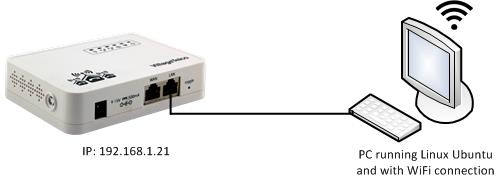
\includegraphics[width=0.8\textwidth]{oppsettviapc}
  \caption [Composition of components during set-up of getting Internet via PC]{\textbf{Composition of components during set-up of getting Internet via PC.} This figure shows how the different components are set-up when the manual for getting Internet via PC is carried out. As shown the PC has a wireless Internet connection.}
  \label{fig:oppsettviapc}
\end{figure}

If you have a PC supporting wireless Internet, there are different ways of getting wireless Internet to it. You can get WiFi on your PC from a router with landline connection, or the PC can establish a wireless connection to a access point for example in form of a cell phone. The cell phone may have a cellular network available. On most new smart phones, you can set your phone to act as an access point (AP), so that other devices can connect to it and get Internet. You can off course connect directly to this AP, but then the MP does not get Internet, and can not spread it further on to several neighbour MPs. The following set-up works for both types; either if you connect to a regular wireless router that gets Internet from for instance xDSL or if you connect to a AP that have a cellular network (3G, 4G) available. 

In order to perform this set up, a PC with Linux Ubuntu with wireless Internet, and a Mesh Potato 2.0 is required. The last octet of the IP address of the MP, is the unique number for each MP. The Mesh Potato is pre-configured with an unique IP address which is stated on the MP. In the following example we use "x" as the last octet. When conducting this description please change the x with the last octet written on your MP.

\begin{enumerate}
\item Connect the MP to the PC, running Linux Ubuntu, with an Ethernet cable. The Ethernet cable must be put into the LAN-port on the MP. 

\item Open Linux terminal and install telnet, dns and iptables by entering the following commands: 
\noindent
\begin{lstlisting}[language=bash]
 $ sudo su
 $ apt-get install telnetd
 $ /etc/init.d/openbsd-inetd restart 
 $ apt-get install dnsmasq
\end{lstlisting}

\item The Mesh Potato will be pre-configured and the IP address 192.168.1.x. In in order to access the MP, the PC must be on the same subnet. To do this write in the terminal: 
\noindent
\begin{lstlisting}[language=bash]
  $ ifconfig eth0 up 192.168.1.2
\end{lstlisting}

\item Open a browser on your PC and type in "192.168.1.x" in the URL field. The SECN Web Interface should now appear. This assures you that you have contact with the Mesh Potato. Changes in the interface will be described further down, so do not close this window.  

\item Go back to the terminal and write the following commands in order to set up the ip tables correctly. You might have to change the "eth0" and "eth1", depending on how your laptop is set up. The eth0 in the following commands is equivalent to the interface of the Ethernet port connected to the MP, while the eth1 is the interface to the wireless network. 
\noindent
\begin{lstlisting}[language=bash]
  $ iptables --table nat --append POSTROUTING --out-interface
   eth1 -j MASQUERADE
  $ iptables --append FORWARD --in-interface eth0 -j ACCEPT
  $ echo 1 > /proc/sys/net/ipv4/ip_forward
\end{lstlisting} 
\begin{itemize}
\item If you mess up in this step, accidentally write something wrong etc., the following commands will reset the ip tables, and you may try step 5 again.
\noindent
\begin{lstlisting}[language=bash]
  $ iptables --table nat --flush
  $ iptables --flush
  $ iptables --delete-chain
\end{lstlisting}
\end{itemize}  

\item Telnet into the \gls{mp} and configure the default gateway by entering the following commands
\begin{lstlisting}[language=bash]
  $ telnet 192.168.1.x
  $ route 
  $ route del default 
  $ route add default gateway 192.168.1.2
\end{lstlisting} 

\item Go back to the web interface and click on the "Advanced"-tab at the top of the page. Change the following parameters under "DHCP Server":
\begin{itemize}
\item Tick the box "Enable DHCP Server".
\item Remove the tick from "Use device IP".
\item Change the address in "Gateway Router" to "192.168.1.2".
\item Press "Save" at the bottom of the page. 
\end{itemize}

\item Internet should now be available in the mesh network. A device can connect to the network with the SSID (name of network) stated on the emergency box. This SSID is also stated in the web interface under "WiFi Access Point".  
\end{enumerate}

\clearpage
\subsubsection{Script providing Internet access via PC}
\label{subsubsec:scriptvipc}

An alternative, and easier method in order to provide Internet access to the \gls{mp} via a PC with WiFi, is running a script. A script is a list of commands that can be executed with less user interactions to automate a process. The script is provided on a USB-stick that is included in the \gls{quick} box. 

A few easy steps must be conducted to run the script:
\begin{enumerate}
\item Connect the MP to the PC (make sure the MP is powered up) running Linux, with an Ethernet cable. The Ethernet cable must be plugged into the LAN-port on the MP.
\item Plug the provided USB-stick into the PC.  
\item Open the terminal on your PC by pressing "Ctrl+Alt+t". 
\item Execute the following commands to enter the right directory (where the script is located):
\noindent
\begin{lstlisting}[language=bash]
  $ sudo su
  $ cd /media/MP-USB
\end{lstlisting}
\item Execute the following command to run the script (Follow the descriptions provided in the script from now on. This information will both be given in the terminal window and as pop-up windows. Make sure you read these carefully):
\noindent
\begin{lstlisting}[language=bash]
  $ sh scriptviaPC.sh
\end{lstlisting}
\item After completing the steps given by the script, Internet access should be available in the mesh network. You can test this by connecting to the \gls{mp} from, for example, your smart phone or a PC. 
\begin{itemize}
\item The name of the network: \textbf{MP2_21}
\item The password is: \textbf{potato-potato}
\end{itemize}
Both the name and the password can be changed in the web interface. 
\end{enumerate}
 
\clearpage
\subsection{Manual for Connecting the MP02 to Satellite}
If you have a satellite dish available, getting Internet to your PC from the dish is not difficult. In addition to the satellite dish, you need a modem, coaxial cable, Ethernet cable and software. Locate the coaxial cable that comes from the dish. After the modem is installed, you plug the coaxial cable to "SATELLITE IN" and "SATELLITE OUT" ports on the modem. Then plug the Ethernet cable to the modem and to your computer. 

So, basically after this is set-up, you can follow the description of how to get Internet to the MP via a PC to get Internet from satellite to the mesh network. 
\clearpage
\section{Training}
The \gls{quick} box are delivered pre-configured, with all the  information necessary to set up a mesh network. It is recommended that the ones using the \gls{quick} box have tested it and tried to set up the network in advance. This to make the process faster and easier when an emergency situation occurs, but it should not be necessary. The provided descriptions should be explanatory and easy enough for most people to use.


\section{How to Create a Network}
The following sections provides some explanation of specific aspects that should be taken into consideration when setting up a network consisting of \glspl{mp} and the \gls{quick} box. 

\subsubsection{Placing the Mesh Potatoes}
The range of the \gls{mp} differs based on terrain. If the terrain is hilly and with many obstacles, the range shortens. It is also important to keep in mind where the \gls{mp}/gls{quick} box is placed. To obtain a longer range, the \glspl{mp} should be placed as high as possible. This could for example be on the roof top, on a telephone pole or any other tall object. With a clear view the range could be up to 2 km. 

\subsubsection{Have a stable power source}
If there is stable power source available there would be no use for the battery and solar panel for charging. In this situation the different pre-configured \glspl{mp} can be spread out, with one connected to an up-link. 

\subsubsection{No stable power source}
It there is no stable power source available there will be a need for the battery and solar panel that is included in the \gls{quick} box in order to run the Mesh Potato. If the power is out there is a high probability that most up-links also are unavailable. Satellite may be the only option. In order to use satellite there have to be a satellite dish available. Keep in mind that this satellite may be located far away, and that there might be a need for several \glspl{mp} in order to spread internet to the desired location. It there is a need for several Mesh Potatoes in an area with power outages there would be a need for several \gls{quick} boxes, so that the \gls{mp} can run on battery charged by a solar panel. 
